% ============================================================================
% Predicción diaria del riesgo de incendio en la Región Pampeana
% Informe final de diplomatura — formato artículo científico.
% Compilar con pdflatex/tectonic (2 pasadas) o subir 06_report/ a Overleaf.
% Las capturas del tablero (figures/dash_*.png) se incorporan automáticamente
% al recompilar si los archivos existen.
% ============================================================================
\documentclass[11pt,a4paper]{article}

\usepackage[utf8]{inputenc}
\usepackage[T1]{fontenc}
\usepackage{lmodern}
\usepackage[spanish,es-tabla]{babel}
\usepackage[margin=2.4cm]{geometry}
\usepackage{graphicx}
\usepackage{booktabs}
\usepackage{amsmath}
\usepackage{float}
\usepackage{placeins}
\usepackage{caption}
\usepackage{microtype}
\usepackage{xcolor}
\usepackage{tikz}
\usetikzlibrary{arrows.meta,positioning,shapes.geometric,calc,decorations.pathreplacing}
\usepackage[colorlinks=true,linkcolor=blue!50!black,citecolor=blue!50!black,urlcolor=blue!50!black]{hyperref}

\captionsetup{font=small,labelfont=bf}
\setlength{\parskip}{1pt}

\title{\textbf{Predicción diaria del riesgo de incendio en la Región Pampeana
mediante XGBoost optimizado por \emph{Sparrow Search Algorithm}, con
calibración de probabilidades y arquitectura \emph{lakehouse} de extremo a
extremo}}
\author{Julián Mendelewicz\\
\small Trabajo final de diplomatura}
\date{Julio de 2026}

\begin{document}
\maketitle

% ----------------------------------------------------------------------------
\begin{abstract}
\noindent
Los incendios de vegetación constituyen una amenaza recurrente para la
producción agropecuaria y los ecosistemas de la Región Pampeana argentina.
Este trabajo presenta un sistema completo de predicción diaria de ocurrencia
de fuego que integra datos satelitales y meteorológicos de múltiples fuentes
sobre una grilla regular de 2.266 celdas de $0{,}25^{\circ}$, cubriendo el
período 2022--2024. Siguiendo el marco propuesto por Wang
\emph{et al.}~\cite{wang2026} para la provincia de Guangdong, se entrenó un
clasificador XGBoost cuyos hiperparámetros fueron optimizados mediante el
\emph{Sparrow Search Algorithm} (SSA), incorporando el sistema canadiense
FWI adaptado al hemisferio sur, variables topográficas, antrópicas, de
vegetación y de autocorrelación espacial. Sobre un conjunto de prueba
temporal estrictamente posterior al entrenamiento (416.024 observaciones,
prevalencia 3,13\,\%), el modelo final alcanzó un AUC-ROC de 0,897 y una
precisión media (AP) de 0,304, superando en 2,4 veces a la persistencia
espacial y en 8,7 veces a un modelo basado únicamente en el índice FWI. El
desarrollo se condujo con criterio de auditoría permanente. Se documentan
cuatro iteraciones del modelo, tres fugas de información detectadas y
corregidas, la recalibración de probabilidades mediante regresión de Platt
(ECE de 0,279 a 0,006) y dos defectos del pipeline de datos descubiertos en
operación gracias a contratos de validación bloqueantes. El sistema se
despliega sobre una arquitectura \emph{lakehouse} con modelado dimensional
en estrella y un tablero analítico orientado a la decisión operativa. Los
resultados indican que el modelo actúa principalmente como un prior
geográfico-estacional modulado por la meteorología del día, conclusión que
se cuantifica mediante análisis SHAP y ablación por bloques de variables.
\medskip

\noindent\textbf{Palabras clave.} predicción de incendios; XGBoost;
\emph{Sparrow Search Algorithm}; calibración de probabilidades; FWI;
arquitectura \emph{lakehouse}; Región Pampeana.
\end{abstract}

% ----------------------------------------------------------------------------
\section{Introducción}
\label{sec:intro}

Los incendios de vegetación representan uno de los riesgos ambientales de
mayor impacto en las regiones templadas productivas. En la Región Pampeana
argentina, la combinación de pastizales naturales, rastrojos agrícolas y
períodos de sequía genera condiciones propicias para igniciones que se
propagan con rapidez, con consecuencias económicas y ecológicas
significativas. La detección satelital de focos activos permite conocer
dónde hay fuego una vez iniciado; la \emph{anticipación} del riesgo, en
cambio, requiere modelos predictivos capaces de estimar la probabilidad de
ocurrencia con antelación suficiente para orientar la vigilancia y la
asignación preventiva de recursos.

La literatura reciente ha demostrado la eficacia de los métodos de
aprendizaje automático basados en árboles potenciados por gradiente para
este problema. Wang \emph{et al.}~\cite{wang2026} integraron detecciones
MODIS con variables meteorológicas, topográficas, de vegetación y
antrópicas para la provincia de Guangdong, y mostraron que un clasificador
XGBoost~\cite{chen2016} cuyos hiperparámetros se optimizan mediante el
\emph{Sparrow Search Algorithm} (SSA)~\cite{xue2020} alcanza un desempeño
superior al de configuraciones ajustadas manualmente, identificando la
pendiente, la proximidad a caminos, la temperatura y la densidad de
población entre los factores determinantes. De manera complementaria, los
sistemas operativos de peligro de incendio se apoyan desde hace décadas en
el \emph{Canadian Forest Fire Weather Index System}
(FWI)~\cite{vanwagner1987}, un conjunto de índices acumulativos de humedad
del combustible que ha sido adaptado a numerosas regiones fuera de Canadá
mediante ajustes en sus tablas estacionales~\cite{lawson2008}.

El presente trabajo adapta el marco de Wang \emph{et al.}\ a un contexto
operativo distinto en tres aspectos. Primero, el dominio corresponde a
pastizales y agroecosistemas del hemisferio sur, lo que exige revisar los
supuestos estacionales del FWI. Segundo, el objetivo no se limita al ajuste
de un clasificador sino a la construcción de un sistema de producción
completo, desde la ingesta diaria de datos hasta un tablero de decisión,
sobre una arquitectura \emph{lakehouse}~\cite{armbrust2021} con garantías de
calidad de datos. Tercero, el desarrollo se condujo bajo un criterio de
auditoría permanente en el que cada iteración del modelo fue examinada en
busca de fugas de información y desalineamientos entre entrenamiento y
servicio, y en el que las métricas publicadas corresponden exclusivamente a
la evaluación limpia posterior a dichas correcciones.

Las contribuciones principales son las siguientes. (i)~Un dataset diario de
riesgo de incendio para la Región Pampeana que integra cinco fuentes
satelitales y meteorológicas sobre una grilla regular, con el sistema FWI
calculado secuencialmente y adaptado al hemisferio sur. (ii)~Un clasificador
XGBoost--SSA evaluado con protocolo estricto de división temporal,
contrastado contra líneas de base no triviales y analizado mediante SHAP,
ablación por bloques y curvas de degradación por horizonte de pronóstico.
(iii)~La recalibración de las probabilidades del modelo mediante regresión
de Platt, requisito para que el valor publicado al usuario final admita una
lectura frecuentista. (iv)~Una arquitectura de datos de tipo \emph{medallion}
con contratos de validación bloqueantes cuya utilidad se demostró
empíricamente al detectar dos defectos latentes durante la puesta en
producción. (v)~Un registro transparente de la evolución del modelo a lo
largo de cuatro versiones, incluyendo las fugas de información detectadas y
el efecto de su corrección sobre las métricas.

El resto del documento se organiza como sigue. La Sección~\ref{sec:datos}
describe el área de estudio, las fuentes y la variable objetivo. La
Sección~\ref{sec:arquitectura} presenta la arquitectura de datos. La
Sección~\ref{sec:metodo} detalla la metodología de modelado y evaluación.
La Sección~\ref{sec:evolucion} documenta la evolución del modelo y los
defectos corregidos. La Sección~\ref{sec:resultados} reporta los
resultados. La Sección~\ref{sec:produccion} describe el despliegue
operativo, y las Secciones~\ref{sec:discusion} y~\ref{sec:conclusiones}
discuten limitaciones y conclusiones.

% ----------------------------------------------------------------------------
\section{Área de estudio y datos}
\label{sec:datos}

\subsection{Área de estudio y unidad de análisis}

El dominio espacial abarca la Región Pampeana y su periferia inmediata,
entre los paralelos $28^{\circ}$S y $42^{\circ}$S y los meridianos
$56^{\circ}$O y $68^{\circ}$O. Sobre ese recuadro se definió una grilla
regular de $0{,}25^{\circ} \times 0{,}25^{\circ}$ (aproximadamente 25~km),
de la cual se retuvieron \textbf{2.266 celdas válidas} tras aplicar una
máscara de tierra firme. Cada celda fue clasificada en una de nueve
subregiones agroecológicas (Pampa Ondulada, Pampa Deprimida, Espinal, Chaco
Húmedo, Chaco Seco, Monte, Delta/Litoral, entre otras) mediante criterios
geográficos. La unidad de observación es el par celda--día y el período de
estudio comprende del 1 de enero de 2022 al 31 de diciembre de 2024, lo que
produce aproximadamente 2,5 millones de observaciones.

\subsection{Variable objetivo}

La variable dependiente es binaria e indica la ocurrencia de al menos una
detección satelital de fuego en vegetación dentro de la celda durante el
día. Se construyó a partir del producto de fuego activo VIIRS de 375~m
distribuido por NASA FIRMS~\cite{firms,schroeder2014}, reteniendo únicamente
detecciones con nivel de confianza nominal o alto y tipo correspondiente a
vegetación, con el fin de excluir falsas alarmas de origen industrial o
reflectivo. Tras la deduplicación y la asignación de cada foco a su celda
más cercana, la prevalencia global resulta cercana al 3\,\% de los pares
celda--día, con fuerte estacionalidad concentrada entre julio y diciembre.

\subsection{Fuentes de datos}

La Tabla~\ref{tab:fuentes} resume las fuentes integradas. La base climática
del entrenamiento proviene del reanálisis ERA5-Land~\cite{era5land},
extraído mediante Google Earth Engine con agregación diaria por celda. Para
la operación diaria se emplea el servicio Open-Meteo, que provee pronóstico
a cuatro días junto con una ventana histórica reciente. La decisión de
utilizar dos proveedores obedece a que el reanálisis ofrece profundidad y
consistencia histórica para entrenar, mientras que el pronóstico operativo
requiere disponibilidad diaria y gratuita; la homogeneización de esquemas
entre ambos se resuelve en la capa de transformación y se valida antes de
cada inferencia.

\begin{table}[H]
\centering\small
\begin{tabular}{@{}llll@{}}
\toprule
\textbf{Fuente} & \textbf{Producto} & \textbf{Resolución} & \textbf{Rol} \\
\midrule
NASA FIRMS & VIIRS 375 m fuego activo & diaria & variable objetivo \\
ERA5-Land (GEE) & reanálisis meteorológico & diaria, $\sim$9 km & clima (entrenamiento) \\
Open-Meteo & pronóstico + histórico & diaria & clima (operación) \\
MODIS MOD13A2 & NDVI compuesto 16 días & 1 km & vegetación \\
MODIS MCD12Q1 & cobertura del suelo anual & 500 m & cobertura \\
OpenStreetMap & red vial & estática & distancia a caminos \\
WorldPop & densidad de población & estática & presión antrópica \\
\bottomrule
\end{tabular}
\caption{Fuentes de datos integradas. Las variables estáticas se
precalcularon por celda en una grilla auxiliar junto con la topografía
(elevación, pendiente y orientación).}
\label{tab:fuentes}
\end{table}

\subsection{Variables predictoras}

El modelo final emplea 39 variables organizadas en siete bloques
(Tabla~\ref{tab:features}). El NDVI de frecuencia 16 días se llevó a
frecuencia diaria mediante propagación del último valor disponible, y su
anomalía se calculó respecto de la media histórica de cada celda,
utilizando exclusivamente el período de entrenamiento para estimar dichas
medias, que se persisten junto al modelo para garantizar consistencia en
servicio. Las variables de autocorrelación espacial siguen el criterio de
contigüidad de reina sobre las ocho celdas vecinas, e incluyen el promedio
y el máximo del FWI del vecindario, así como un indicador de ocurrencia de
fuego en el vecindario durante los tres días previos con ventana
estrictamente retrospectiva.

\begin{table}[H]
\centering\small
\begin{tabular}{@{}llc@{}}
\toprule
\textbf{Bloque} & \textbf{Variables} & \textbf{N} \\
\midrule
Estáticas & subregión, elevación, pendiente, orientación, & 7 \\
 & dist.\ a caminos, densidad poblacional, cobertura & \\
Meteorología & temperatura, HR, viento, precipitación, radiación, & 12 \\
 & humedad de suelo (2 capas), VPD, días secos, & \\
 & z-score de precipitación 90 d, medias móviles 30 d (2) & \\
Sistema FWI & FFMC, DMC, ISI, BUI, FWI, medias móviles 14/30 d & 7 \\
Vegetación & NDVI, anomalía de NDVI por celda & 2 \\
Estacionalidad & sen/cos de mes y día del año, calendario agrícola & 5 \\
Interacciones & FWI$\times$VPD, temp.$\times$días secos, viento$\times$FWI & 3 \\
Espaciales & FWI vecinal (media, máx.), fuego vecinal 3 días & 3 \\
\midrule
\textbf{Total} & & \textbf{39} \\
\bottomrule
\end{tabular}
\caption{Bloques de variables predictoras del modelo final. La partición en
bloques es la utilizada en el análisis de ablación de la
Sección~\ref{sec:shap}.}
\label{tab:features}
\end{table}

% ----------------------------------------------------------------------------
\section{Arquitectura del sistema de datos}
\label{sec:arquitectura}

\subsection{Pipeline \emph{medallion}}

El sistema se implementó sobre Databricks siguiendo el patrón
\emph{lakehouse}~\cite{armbrust2021} con arquitectura \emph{medallion} de
cuatro capas (Figura~\ref{fig:medallion}). La capa \emph{landing} recibe los
archivos crudos de cada fuente en volúmenes de Unity Catalog. La capa
\emph{bronze} realiza la ingesta incremental mediante Auto Loader con
puntos de control idempotentes, preservando metadatos de linaje (archivo de
origen y marca temporal de ingesta). La capa \emph{silver} aplica la
limpieza tipada por fuente, y la capa \emph{gold} materializa los datasets
de consumo tanto para el entrenamiento como para la inferencia diaria y la
capa analítica.

\begin{figure}[H]
\centering
\begin{tikzpicture}[
  capa/.style={draw=black!35, rounded corners=2.5pt, minimum height=12mm,
               minimum width=25mm, align=center, inner sep=3pt},
  flecha/.style={-{Stealth[length=2.6mm]}, semithick, draw=black!55},
  nota/.style={font=\scriptsize\itshape, text=black!60},
]
  \node[capa, fill=black!5]
    (landing) {\textbf{\small Landing}\\[1pt]\scriptsize CSV en Volumes};
  \node[capa, fill=brown!20, right=7mm of landing]
    (bronze) {\textbf{\small Bronze}\\[1pt]\scriptsize Delta $\cdot$ Auto Loader};
  \node[capa, fill=black!13, right=7mm of bronze]
    (silver) {\textbf{\small Silver}\\[1pt]\scriptsize limpieza $\cdot$ contratos};
  \node[capa, fill=yellow!30, right=7mm of silver]
    (gold)   {\textbf{\small Gold}\\[1pt]\scriptsize OBT (ML) $\cdot$ estrella (BI)};
  \node[capa, fill=blue!11, right=7mm of gold]
    (consumo){\textbf{\small Consumo}\\[1pt]\scriptsize modelo $\cdot$ tablero};

  \draw[flecha] (landing) -- (bronze);
  \draw[flecha] (bronze)  -- (silver);
  \draw[flecha] (silver)  -- (gold);
  \draw[flecha] (gold)    -- (consumo);

  \draw[decorate, decoration={brace, mirror, amplitude=4pt}, draw=black!45]
    ($(landing.south west)+(0,-2mm)$) -- ($(consumo.south east)+(0,-2mm)$)
    node[midway, below=6pt, nota]
    {Job diario serverless — 7 tareas encadenadas, idempotente, 06:00 UTC};
\end{tikzpicture}
\caption{Arquitectura \emph{medallion} sobre Databricks con Unity Catalog y
tablas Delta. El mismo pipeline sirve al entrenamiento (histórico
2022--2024) y a la operación diaria (ventana de 35 días observados más 4 de
pronóstico).}
\label{fig:medallion}
\end{figure}

\subsection{Estándares y contratos de la capa \emph{silver}}
\label{sec:silver}

La capa \emph{silver} se ajustó a prácticas estándar de la industria. Las
tablas siguen la convención de nombres \texttt{silver\_<fuente>}, se
deduplican por clave natural (celda y fecha) y aplican recortes de dominio
físico, dado que los proveedores producen ocasionalmente valores imposibles
por artefactos de agregación, tales como precipitaciones de $-0{,}00$~mm,
humedades relativas superiores al 100\,\% o valores de NDVI fuera del
intervalo $[-1,1]$. Todas las tablas incorporan una columna de linaje con
la marca temporal de procesamiento.

Además de la auditoría descriptiva posterior a la carga, la transformación
diaria incorpora \textbf{contratos de datos bloqueantes} que se verifican
antes de cada escritura. Se exige la completitud de nodos respecto de la
grilla de referencia, la unicidad de la clave natural, la pertenencia de
las variables a sus rangos físicos, la ausencia de valores nulos en los
índices FWI y una profundidad mínima de la ventana histórica. Cuando un
contrato falla, la tarea aborta con un mensaje diagnóstico y las etapas
posteriores no se ejecutan, de modo que un dato defectuoso no puede
propagarse hasta las predicciones publicadas. La Sección~\ref{sec:defectos}
documenta dos defectos reales que este mecanismo permitió detectar y que
habrían pasado inadvertidos bajo un esquema de auditoría puramente
descriptiva.

\subsection{Capa \emph{gold} con doble modelado}
\label{sec:estrella}

La capa \emph{gold} combina dos representaciones complementarias. Para el
aprendizaje automático se materializan tablas anchas de tipo \emph{one big
table}, una para el entrenamiento histórico y otra para la inferencia
diaria, en las que cada fila constituye un ejemplo con las 39 variables
listas para el clasificador. Esta representación es la interfaz natural de
un modelo de árboles potenciados y su contenido queda ligado al modelo por
la suma de verificación del dataset.

Para el consumo analítico se agregó un \textbf{esquema en estrella}
conforme a la metodología dimensional de Kimball~\cite{kimball}, ilustrado
en la Figura~\ref{fig:estrella} y descrito en la Tabla~\ref{tab:estrella}.
El hecho central registra las predicciones con grano celda por fecha de
pronóstico por corrida, lo que otorga idempotencia a la inferencia diaria y
conserva el historial de corridas. Las dimensiones concentran los atributos
descriptivos y evitan su repetición en los hechos. Dos hechos secundarios
registran la meteorología diaria y las detecciones históricas de fuego, y
dos tablas auxiliares exponen la importancia de variables y las métricas de
líneas de base para la página analítica del tablero. La integridad
referencial entre dimensiones y hechos se verifica mediante aserciones en
cada corrida, dado que el formato de tablas subyacente no la impone por sí
mismo. Se optó deliberadamente por mantener ambas representaciones en lugar
de reemplazar una por otra, puesto que sirven a consumidores con ciclos de
vida distintos; la tabla ancha es el contrato del modelo y la estrella es el
contrato del tablero.

\begin{table}[H]
\centering\small
\begin{tabular}{@{}lll@{}}
\toprule
\textbf{Tabla} & \textbf{Grano} & \textbf{Fuente} \\
\midrule
\texttt{dim\_cell} & celda de grilla & grilla auxiliar + cobertura \\
\texttt{dim\_date} & día calendario 2022--2027 & generada \\
\texttt{dim\_model} & versión de modelo & artefactos de evaluación \\
\texttt{fact\_prediction} & celda $\times$ fecha pron.\ $\times$ corrida & motor de inferencia \\
\texttt{fact\_weather\_daily} & celda $\times$ día (35 obs.\ + 4 pron.) & \texttt{silver\_openmeteo} \\
\texttt{fact\_fire\_detection} & celda $\times$ día con focos & \texttt{silver\_nasa\_firms} \\
\texttt{fact\_feature\_importance} & variable $\times$ modelo & análisis SHAP \\
\texttt{fact\_baseline\_metrics} & línea de base $\times$ modelo & evaluación \\
\bottomrule
\end{tabular}
\caption{Esquema en estrella de la capa de presentación. Dos vistas
(\texttt{vw\_predictions\_latest}, \texttt{vw\_fire\_history}) resuelven las
uniones habituales para el tablero.}
\label{tab:estrella}
\end{table}

\begin{figure}[H]
\centering
\begin{tikzpicture}[
  dim/.style={draw=blue!40!black!45, rounded corners=2.5pt, fill=blue!8,
              minimum height=11mm, minimum width=32mm, align=center,
              font=\scriptsize, inner sep=3pt},
  factsec/.style={draw=orange!50!black!30, rounded corners=2.5pt,
                  fill=orange!6, minimum height=9mm, minimum width=29mm,
                  align=center, font=\tiny, inner sep=2.5pt},
  rayo/.style={draw=orange!55!black!70, line width=1.1pt},
  lineasec/.style={draw=black!25, thin, dashed},
]
  % Rayos de la estrella (debajo de los nodos)
  \draw[rayo] (0,0) -- (-4.9,  2.35);   % a dim_cell
  \draw[rayo] (0,0) -- ( 4.9,  2.35);   % a dim_date
  \draw[rayo] (0,0) -- ( 0,    2.6);    % a dim_model
  \draw[rayo] (0,0) -- (-4.9, -2.35);   % a dim_subrol izq (weather via cell)
  \draw[rayo] (0,0) -- ( 4.9, -2.35);   % rayo inferior derecho

  % Dimensiones en las puntas superiores y laterales
  \node[dim] (cell)  at (-4.9,  2.35) {\textbf{dim\_cell}\\[1pt] lat/lon $\cdot$ subregión $\cdot$ cobertura};
  \node[dim] (model) at ( 0,    2.6)  {\textbf{dim\_model}\\[1pt] AUC $\cdot$ AP $\cdot$ ECE $\cdot$ umbrales};
  \node[dim] (date)  at ( 4.9,  2.35) {\textbf{dim\_date}\\[1pt] estación austral $\cdot$ temporada};

  % Hechos secundarios en las puntas inferiores (subordinados)
  \node[factsec] (weather) at (-4.9, -2.35) {\textbf{fact\_weather\_daily}\\[1pt] clima + FWI (35d + 4d)};
  \node[factsec] (fire)    at ( 4.9, -2.35) {\textbf{fact\_fire\_detection}\\[1pt] focos VIIRS 2022--2024};

  % Hecho central — el corazón de la estrella
  \node[draw=orange!75!black!65, very thick, rounded corners=3pt,
        fill=orange!24, minimum height=14mm, minimum width=40mm,
        align=center, font=\small, inner sep=4pt] (pred) at (0,0)
    {\textbf{fact\_prediction}\\[2pt]
     \scriptsize prob.\ calibrada $\cdot$ percentil $\cdot$ alerta};

  % Los hechos secundarios comparten dimensiones (relaciones punteadas)
  \draw[lineasec] (weather.north) -- (cell.south);
  \draw[lineasec] (fire.north)    -- (date.south);
  \draw[lineasec] (weather.east) to[bend right=10] (date.south west);
  \draw[lineasec] (fire.west)    to[bend left=10]  (cell.south east);
\end{tikzpicture}
\caption{Esquema en estrella de la capa de presentación. El hecho central
\texttt{fact\_prediction} irradia hacia las puntas de la estrella; las
puntas superiores son las dimensiones y las inferiores los hechos
secundarios, que comparten \texttt{dim\_cell} y \texttt{dim\_date}
(relaciones punteadas). Se omiten las tablas de importancia y de líneas de
base, relacionadas únicamente con \texttt{dim\_model}.}
\label{fig:estrella}
\end{figure}

\subsection{Orquestación}

Un \emph{job} diario de Databricks sobre cómputo \emph{serverless},
programado a las 06:00~UTC, encadena siete tareas. Las dos primeras extraen
de Open-Meteo el pronóstico a cuatro días y la ventana histórica de 35
días. Las siguientes realizan la ingesta a \emph{bronze}, la transformación
\emph{silver} con sus contratos, la construcción de la tabla de inferencia
con las 39 variables alineadas al entrenamiento, la inferencia propiamente
dicha y el refresco del esquema en estrella. La inferencia es idempotente
por corrida, en el sentido de que una reejecución dentro del mismo día
reemplaza la corrida previa en lugar de duplicarla.

% ----------------------------------------------------------------------------
\section{Metodología}
\label{sec:metodo}

\subsection{Sistema FWI adaptado al hemisferio sur}
\label{sec:fwi}

El sistema FWI~\cite{vanwagner1987} modela la humedad de tres estratos de
combustible mediante los códigos FFMC, DMC y DC, de los que derivan los
índices de propagación ISI, de combustible disponible BUI y el índice
integrado FWI. El cálculo es secuencial por celda, dado que el estado de
cada día depende del anterior, y se implementó en un módulo compartido por
el entrenamiento y la operación para garantizar la identidad de ambas
trayectorias.

La adaptación al hemisferio sur exigió desplazar seis meses las tablas
estacionales de longitud efectiva del día, siguiendo los valores publicados
para latitudes de 30--40$^{\circ}$S~\cite{lawson2008}. Durante el
desarrollo se detectó que una versión previa empleaba por error la tabla
$L_f$ del código DC, que toma valores negativos en invierno, para el
cálculo del DMC, lo que colapsaba dicho código durante todo el invierno
austral en contradicción con la física del modelo; la versión corregida
emplea la tabla $L_e$ correspondiente, de valores siempre positivos. Dado
que los códigos DMC y DC convergen lentamente desde sus valores iniciales
convencionales (FFMC~85, DMC~6, DC~15), el entrenamiento descarta las
primeras ocho semanas del período como fase de estabilización, y la
operación diaria garantiza la continuidad del cálculo manteniendo una
ventana histórica deslizante de 35 días previa al pronóstico.

\subsection{Diseño experimental}
\label{sec:split}

La evaluación adopta una división temporal estricta en tres particiones. El
conjunto de entrenamiento comprende desde marzo de 2022 hasta abril de 2024
y se balancea a razón 1:1 mediante submuestreo estratificado por subregión,
lo que produce 81.212 ejemplos. El conjunto de validación cubre mayo y
junio de 2024 con su distribución natural (137.921 observaciones) y se
emplea para la detención temprana, la calibración y la selección de
umbrales. El conjunto de prueba, estrictamente posterior, abarca de julio a
diciembre de 2024 (416.024 observaciones, prevalencia 3,13\,\%) y coincide
con la temporada de fuego; ninguna decisión de modelado se tomó con
información de esta partición. La reproducibilidad se asegura persistiendo
la suma MD5 del dataset y la semilla aleatoria junto con las métricas, y la
suite de evaluación verifica en cada ejecución que el modelo publicado
reproduce el AUC de referencia con deriva nula.

El balanceo del entrenamiento responde a la baja prevalencia del fenómeno,
pero introduce una distorsión conocida en las probabilidades del modelo,
que quedan referidas a un universo con prevalencia artificial del 50\,\%.
La Sección~\ref{sec:calibracion} trata la corrección de este efecto, y se
señala asimismo que la métrica AP utilizada durante la búsqueda de
hiperparámetros, calculada por validación cruzada sobre el conjunto
balanceado, opera en ese universo distorsionado y no es comparable con el
AP reportado sobre el conjunto de prueba.

\subsection{Optimización de hiperparámetros mediante SSA}
\label{sec:ssa}

El \emph{Sparrow Search Algorithm}~\cite{xue2020} es un metaheurístico
poblacional inspirado en el comportamiento de forrajeo y vigilancia de los
gorriones, en el que la población se divide en productores, que exploran el
espacio de búsqueda, y rastreadores, que explotan las mejores soluciones,
con un subconjunto de individuos centinela que introduce perturbaciones
ante el riesgo de estancamiento. Siguiendo a Wang \emph{et al.}, se empleó
SSA para optimizar ocho hiperparámetros de XGBoost, con una población de 15
individuos y 15 iteraciones, deteniendo la búsqueda ante ausencia de mejora
sostenida. La función objetivo fue la precisión media obtenida por
validación cruzada de tres particiones sobre el conjunto de entrenamiento
balanceado. La configuración resultante se reporta en la
Tabla~\ref{tab:hiperparametros}; el modelo final emplea 237 árboles
seleccionados por detención temprana sobre la partición de validación.

\begin{table}[H]
\centering\small
\begin{tabular}{@{}lc@{}}
\toprule
\textbf{Hiperparámetro} & \textbf{Valor} \\
\midrule
Profundidad máxima & 8 \\
Tasa de aprendizaje & 0,0519 \\
Submuestreo de filas & 0,791 \\
Submuestreo de columnas & 0,840 \\
Peso mínimo por hoja & 6 \\
$\gamma$ (poda) & 1,447 \\
Regularización $L_1$ ($\alpha$) & 3,024 \\
Regularización $L_2$ ($\lambda$) & 1,399 \\
Árboles (detención temprana) & 237 \\
\bottomrule
\end{tabular}
\caption{Hiperparámetros del modelo final obtenidos por SSA (15 individuos,
15 iteraciones, validación cruzada de 3 particiones sobre el conjunto
balanceado).}
\label{tab:hiperparametros}
\end{table}

\subsection{Calibración de probabilidades}
\label{sec:calibracion}

Un sistema de alerta que publica probabilidades debe garantizar que estas
admitan lectura frecuentista, esto es, que entre los casos a los que asigna
un valor $p$ la fracción observada de positivos sea aproximadamente $p$. La
desviación se cuantifica mediante el error de calibración esperado,

\begin{equation}
\mathrm{ECE} = \sum_{b=1}^{B} \frac{n_b}{N}\,
\bigl|\, \bar{p}_b - \bar{y}_b \,\bigr|,
\label{eq:ece}
\end{equation}

\noindent donde la predicción se particiona en $B$ intervalos de igual
población, $\bar{p}_b$ es la probabilidad media predicha en el intervalo
$b$ y $\bar{y}_b$ la fracción de positivos observada. El modelo crudo
presenta un ECE de 0,279 sobre el conjunto de prueba, consecuencia directa
del entrenamiento balanceado descrito en la Sección~\ref{sec:split};
cuando el modelo predice un 60\,\% la frecuencia observada ronda el 5\,\%.

Se compararon dos correctores ajustados sobre la partición de validación.
La regresión isotónica~\cite{zadrozny2002} y el escalado de
Platt~\cite{platt1999}, que ajusta una transformación sigmoidea

\begin{equation}
\hat{p} = \sigma\!\bigl(a \cdot \mathrm{logit}(p) + b\bigr),
\label{eq:platt}
\end{equation}

\noindent con $a$ y $b$ estimados por máxima verosimilitud. Ambos reducen
el ECE en dos órdenes de magnitud, pero la isotónica, al ser una función
escalonada, empata bloques de puntuaciones y degrada la precisión media de
0,304 a 0,284, mientras que la transformación de Platt es estrictamente
monótona y preserva el ordenamiento de manera exacta, con AUC y AP
idénticos al modelo crudo. Se adoptó por lo tanto el escalado de Platt, con
un ECE final de 0,006. En servicio, el corrector se evalúa a partir de sus
coeficientes serializados en un archivo de texto, evitando la
deserialización de objetos dependientes de versiones de biblioteca en el
entorno de inferencia.

El umbral operativo se rederivó sobre las probabilidades calibradas
maximizando la medida $F_{\beta}$ con $\beta=2$ en validación, elección que
prioriza la exhaustividad por sobre la precisión en atención a la asimetría
de costos del dominio, donde omitir un fuego real resulta más costoso que
emitir una falsa alarma. El umbral resultante es $\tau = 0{,}070$, con
exhaustividad de 0,634 y precisión de 0,218 sobre el conjunto de prueba.

\subsection{Protocolo de evaluación}
\label{sec:protocolo}

El desempeño se contrasta contra tres líneas de base. La primera predice
constantemente la prevalencia. La segunda es la persistencia espacial, que
asigna riesgo positivo a las celdas con fuego observado en los tres días
previos, y constituye el competidor natural de un sistema de vigilancia.
La tercera es un XGBoost entrenado únicamente con el índice FWI, que
representa la práctica operativa tradicional basada en peligro
meteorológico. La interpretación del modelo emplea valores
SHAP~\cite{lundberg2017} en lugar de la importancia por ganancia del propio
XGBoost, cuyo sesgo hacia variables de corte frecuente se discute en la
Sección~\ref{sec:shap}, y se complementa con una ablación por bloques que
reentrena el modelo excluyendo cada grupo de la Tabla~\ref{tab:features}.
Finalmente, se cuantifica la degradación por horizonte de pronóstico
simulando el estado real de servicio, en el que el indicador de fuego
vecinal no es observable para horizontes mayores a un día, y se examina la
heterogeneidad espacial del error por subregión.

% ----------------------------------------------------------------------------
\section{Evolución del modelo y defectos corregidos}
\label{sec:evolucion}

El desarrollo atravesó cuatro versiones del modelo y dos auditorías
integrales del código, una durante el desarrollo y otra previa a la puesta
en producción. Esta sección documenta ese recorrido, en el entendimiento de
que la transparencia sobre los errores cometidos y corregidos forma parte
del rigor metodológico del trabajo.

\subsection{De la línea de base al modelo final}
\label{sec:versiones}

La Tabla~\ref{tab:versiones} resume las cuatro iteraciones. La primera
versión entrenó sobre la distribución natural sin balanceo y con una
búsqueda de hiperparámetros preliminar; con el umbral elegido alcanzaba una
exhaustividad de 0,965 a costa de una precisión del 3\,\%, es decir,
alertaba sobre la práctica totalidad de la región, comportamiento inútil a
efectos operativos. La segunda versión introdujo el balanceo 1:1
estratificado por subregión, la optimización SSA completa y las variables
de interacción, elevando la precisión media de 0,181 a 0,295. La tercera
versión refinó la detención temprana y la infraestructura de entrenamiento,
alcanzando una precisión media de 0,315. La cuarta versión incorporó las
variables de autocorrelación espacial y, de manera decisiva, corrigió las
fugas de información descritas a continuación, por lo que sus métricas son
las únicas directamente comparables con un despliegue real.

\begin{table}[H]
\centering\small
\begin{tabular}{@{}lllcc@{}}
\toprule
\textbf{Versión} & \textbf{Cambios principales} & \textbf{Estado} & \textbf{AUC} & \textbf{AP} \\
\midrule
v1 & sin balanceo, SSA preliminar & con fugas & 0,863 & 0,181 \\
v2 & balanceo 1:1, SSA completo, interacciones & con fugas & 0,893 & 0,295 \\
v3 & detención temprana con paciencia, refactor & con fugas & 0,898 & 0,315 \\
v4 & variables espaciales, corrección de fugas & \textbf{limpio} & \textbf{0,897} & \textbf{0,304} \\
\bottomrule
\end{tabular}
\caption{Evolución del modelo. Las métricas de v1--v3 están infladas por las
fugas de información posteriormente detectadas y no son comparables entre
sí en sentido estricto; se reportan como registro del proceso. El AUC de v4
es marginalmente inferior al de v3 precisamente porque elimina información
ilegítima.}
\label{tab:versiones}
\end{table}

\subsection{Fugas de información detectadas y corregidas}
\label{sec:fugas}

La auditoría del código de entrenamiento identificó tres mecanismos de fuga
de información, todos corregidos en la versión final.

La primera fuga afectaba a la anomalía de NDVI, que se calculaba como
desviación respecto de la media de cada celda computada sobre el
\emph{dataset completo}, incluyendo los períodos de validación y prueba. La
corrección restringe el cálculo de las medias al período de entrenamiento y
las persiste como artefacto del modelo, de modo que el servicio utilice
exactamente los mismos valores.

La segunda fuga consistía en emplear el conjunto de prueba como conjunto de
evaluación para la detención temprana del entrenamiento, práctica que
selecciona implícitamente el número de árboles que maximiza el desempeño en
prueba. La corrección introduce la partición de validación intermedia
descrita en la Sección~\ref{sec:split}, reservando la prueba para un único
uso final.

La tercera fuga involucraba al indicador de fuego vecinal, cuya ventana
temporal incluía el propio día de la predicción, con lo cual la variable
incorporaba información contemporánea al evento que se pretendía predecir.
La corrección impone una ventana estrictamente retrospectiva sobre los tres
días previos, idéntica en entrenamiento y servicio.

El efecto conjunto de estas correcciones se aprecia en la
Tabla~\ref{tab:versiones}. El AUC desciende de 0,898 a 0,897 y la precisión
media de 0,315 a 0,304 al pasar de la versión con fugas a la versión
limpia, a pesar de que esta última agrega variables espaciales de valor
genuino. La magnitud moderada del descenso indica que las fugas inflaban
las métricas de manera perceptible pero no dominante; su corrección importa
menos por el tamaño del ajuste que por la validez de las cifras publicadas.

\subsection{Defectos del pipeline detectados en operación}
\label{sec:defectos}

Dos defectos adicionales emergieron durante la puesta en producción del
pipeline diario, y su detección ilustra el valor de los contratos de datos
de la Sección~\ref{sec:silver}.

El primero afectaba a la ventana histórica meteorológica. El extractor del
histórico estaba concebido para ejecutarse una única vez en la
inicialización del sistema, mientras que la retención de la capa
\emph{bronze} eliminaba diariamente los registros con antigüedad mayor a 35
días. En consecuencia, la ventana se acortaba un día por cada jornada de
operación hasta vaciarse por completo, dejando al cálculo del FWI sin fase
de estabilización, todo ello mientras cada tarea del pipeline reportaba
ejecución exitosa. El defecto se detectó al verificar los conteos del
esquema en estrella, cuya tabla de hechos meteorológicos contenía
únicamente los cuatro días de pronóstico. La corrección convirtió la
extracción del histórico en una operación diaria que reconstruye la ventana
completa, y añadió al contrato de la capa \emph{silver} la exigencia de una
profundidad histórica mínima, de manera que una regresión futura de este
tipo aborte el pipeline en lugar de degradar silenciosamente las
predicciones.

El segundo defecto residía en la implementación del índice BUI. Ante
valores simultáneamente bajos de los códigos DMC y DC, situación
característica del invierno austral con precipitación intensa y bajas
temperaturas, la segunda rama de la ecuación del BUI produce valores
negativos, y la potencia fraccionaria $\mathrm{BUI}^{0{,}809}$ del cálculo
posterior del FWI degenera entonces en un valor indefinido. La
implementación de referencia del sistema canadiense acota el BUI
inferiormente en cero, salvaguarda que faltaba en la implementación propia
y que se incorporó en el módulo compartido. Cabe señalar que el defecto
permaneció latente durante todo el entrenamiento, dado que las secuencias
meteorológicas del período histórico no alcanzaron la región crítica del
espacio de estados, y se manifestó recién ante la primera ventana operativa
de invierno con datos reales completos, donde fue interceptado por el
contrato que exige la no nulidad de los índices FWI.

% ----------------------------------------------------------------------------
\section{Resultados}
\label{sec:resultados}

\subsection{Desempeño global y comparación con líneas de base}

Sobre el conjunto de prueba, el modelo final alcanza un AUC-ROC de 0,8965 y
una precisión media de 0,3038. La Tabla~\ref{tab:baselines} sitúa estas
cifras en contexto. La persistencia espacial, competidor serio en un
fenómeno con fuerte autocorrelación, obtiene una precisión media de 0,125,
por lo que el modelo la multiplica por 2,4. El modelo entrenado únicamente
con el índice FWI apenas supera a la predicción por prevalencia (0,035
frente a 0,031), resultado que merece subrayarse por su implicancia
operativa. El índice de peligro meteorológico estándar de la disciplina,
empleado de manera aislada, carece de capacidad discriminante sobre
\emph{dónde} ocurrirá el fuego en la región de estudio; su información es
predominantemente temporal, mientras que la señal espacial reside en la
geografía y la presión antrópica.

\begin{table}[H]
\centering\small
\begin{tabular}{@{}lcc@{}}
\toprule
\textbf{Modelo} & \textbf{AUC} & \textbf{AP} \\
\midrule
Prevalencia constante & 0,500 & 0,031 \\
Solo FWI (XGBoost univariado) & 0,552 & 0,035 \\
Persistencia espacial (3 días) & 0,719 & 0,125 \\
\textbf{Modelo final (39 variables)} & \textbf{0,897} & \textbf{0,304} \\
\bottomrule
\end{tabular}
\caption{Comparación contra líneas de base sobre el conjunto de prueba
(416.024 observaciones, prevalencia 3,13\,\%).}
\label{tab:baselines}
\end{table}

\begin{figure}[H]
\centering
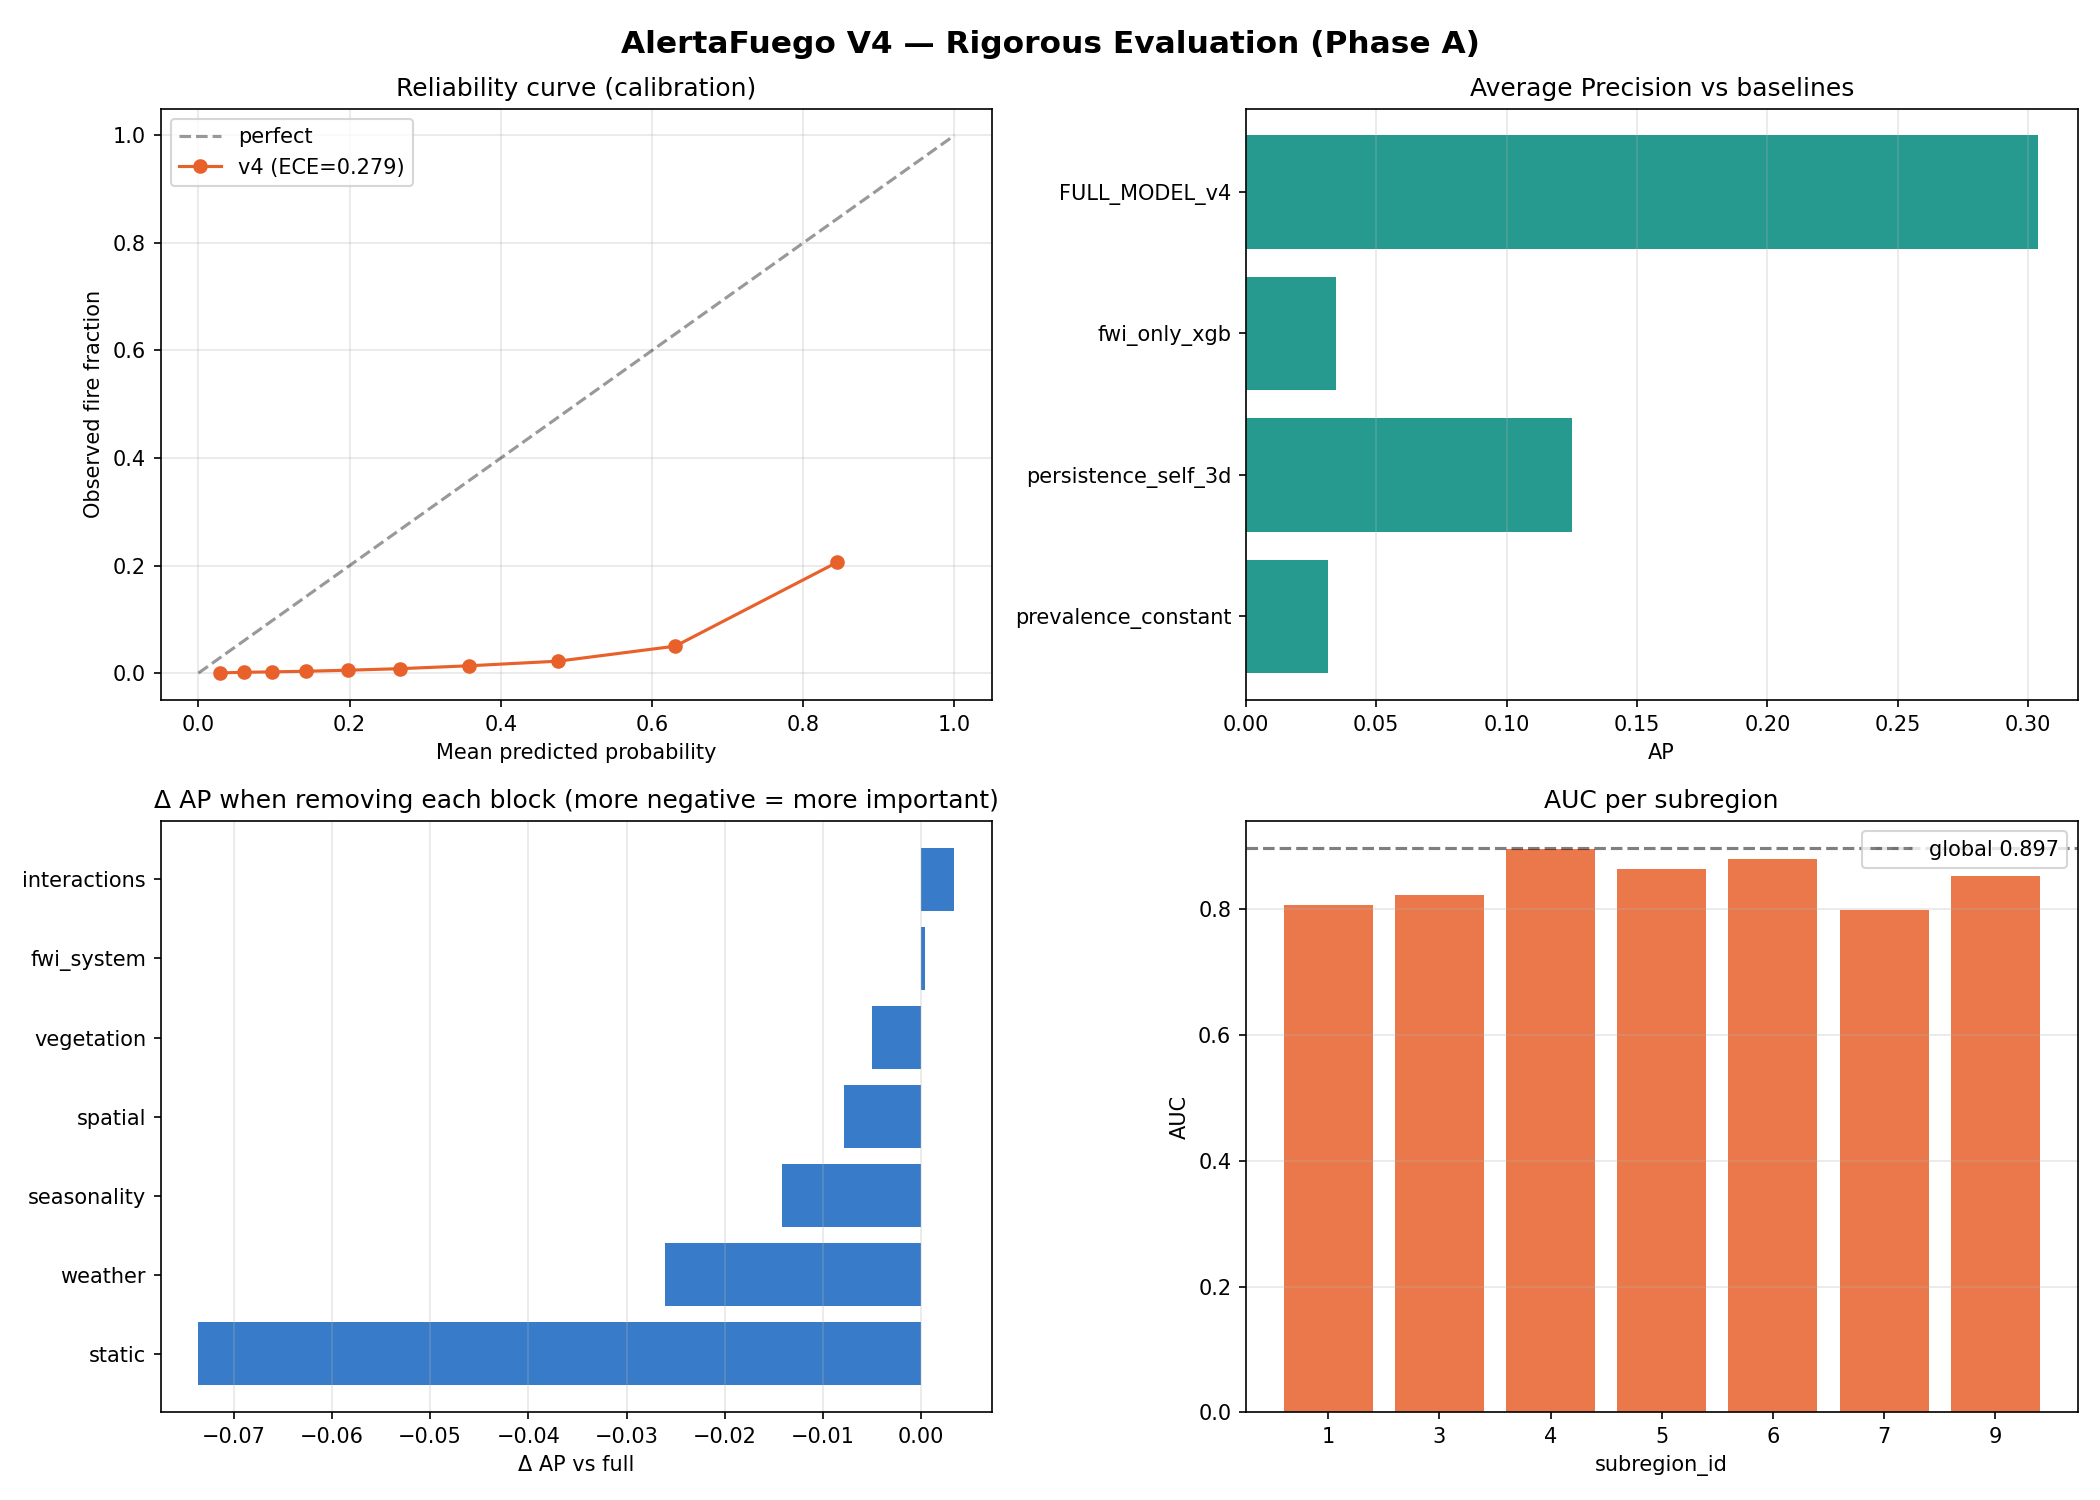
\includegraphics[width=\textwidth]{figures/eval_plots_v4.png}
\caption{Suite de evaluación del modelo final. Arriba a la izquierda, curva
de fiabilidad del modelo sin calibrar (ECE 0,279), que motiva la corrección
de la Sección~\ref{sec:calibracion}. Arriba a la derecha, precisión media
contra líneas de base. Abajo a la izquierda, ablación por bloques
($\Delta$AP al excluir cada bloque). Abajo a la derecha, AUC por subregión.}
\label{fig:eval}
\end{figure}

\subsection{Calibración}

La Figura~\ref{fig:calibracion} muestra la curva de fiabilidad tras aplicar
el escalado de Platt. El ECE desciende de 0,279 a 0,0056 sin alteración
alguna del ordenamiento, conforme a lo discutido en la
Sección~\ref{sec:calibracion}, y la comparación con la regresión isotónica
(Tabla~\ref{tab:calibracion}) fundamenta la elección del método. Tras la
calibración, la probabilidad publicada por el sistema admite lectura
directa; un valor del 5\,\% corresponde a una frecuencia observada cercana
al 5\,\%.

\begin{table}[H]
\centering\small
\begin{tabular}{@{}lcccc@{}}
\toprule
\textbf{Corrector} & \textbf{ECE val.} & \textbf{ECE prueba} & \textbf{AUC} & \textbf{AP} \\
\midrule
Sin calibrar & 0,191 & 0,279 & 0,8965 & 0,3038 \\
Regresión isotónica & $\approx 0$ & 0,0061 & 0,8959 & 0,2838 \\
\textbf{Platt (adoptado)} & 0,0007 & \textbf{0,0056} & \textbf{0,8965} & \textbf{0,3038} \\
\bottomrule
\end{tabular}
\caption{Comparación de correctores de calibración ajustados sobre
validación y evaluados sobre prueba. La transformación de Platt corrige el
ECE preservando el ordenamiento de manera exacta.}
\label{tab:calibracion}
\end{table}

\begin{figure}[H]
\centering
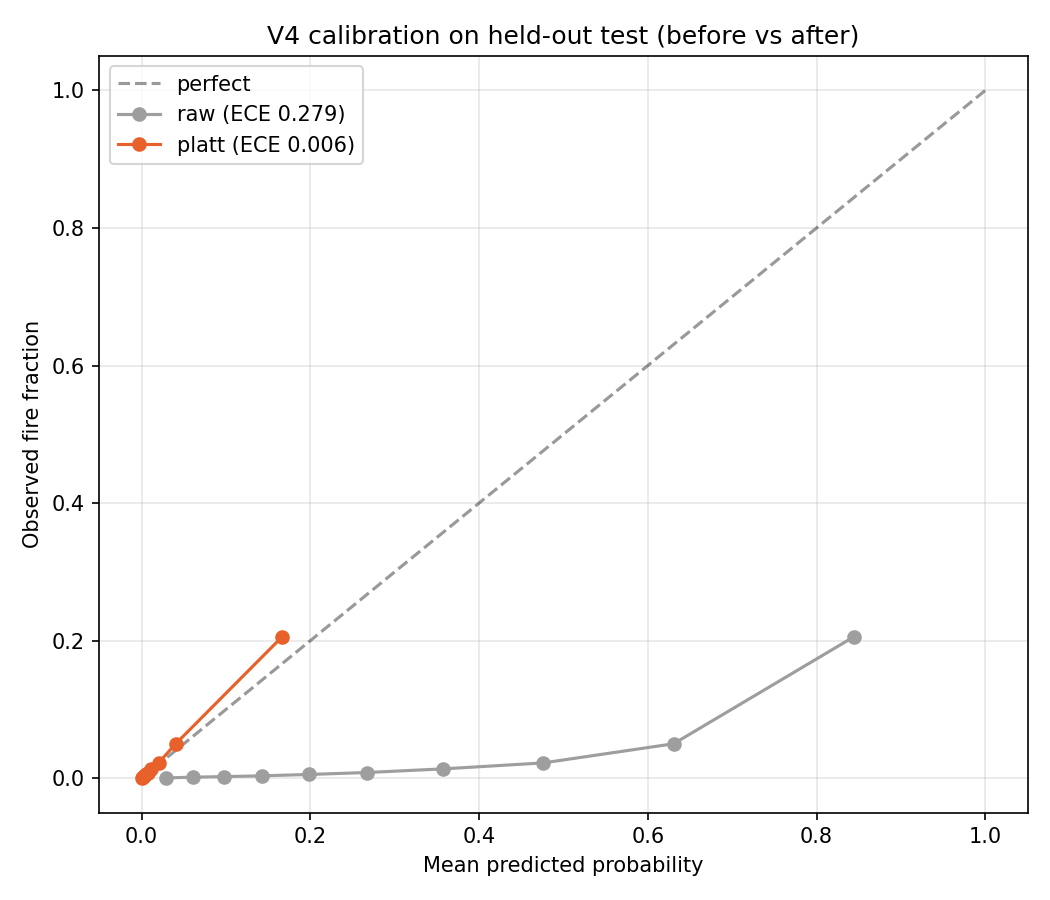
\includegraphics[width=0.58\textwidth]{figures/calibration_v4_after.png}
\caption{Curva de fiabilidad tras el escalado de Platt. La probabilidad
predicha coincide con la frecuencia observada a lo largo de todo el rango.}
\label{fig:calibracion}
\end{figure}

\subsection{Importancia de variables y ablación por bloques}
\label{sec:shap}

La importancia por ganancia del propio XGBoost atribuía el 73\,\% del total
al indicador de fuego vecinal, lectura que sugería un modelo de puro
contagio espacial. El análisis SHAP corrige sustancialmente esa
interpretación (Tabla~\ref{tab:shap}). El indicador vecinal conserva el
primer puesto pero con un peso comparable al de la elevación, y el grueso
de la contribución se distribuye entre las variables estáticas, la
radiación solar y la estacionalidad. La discrepancia entre ambos rankings
ilustra el sesgo conocido de la importancia por ganancia hacia variables
utilizadas en cortes tempranos y frecuentes, y justifica la adopción de
SHAP como criterio interpretativo del sistema.

\begin{table}[H]
\centering\small
\begin{tabular}{@{}rlcc@{}}
\toprule
\# & \textbf{Variable} & \textbf{SHAP $\overline{|v|}$} & \textbf{Ganancia} \\
\midrule
1 & fuego vecinal 3 días & 0,522 & 0,733 \\
2 & elevación & 0,498 & 0,021 \\
3 & densidad de población & 0,326 & 0,012 \\
4 & radiación solar & 0,320 & 0,008 \\
5 & coseno del día del año & 0,273 & 0,006 \\
6 & subregión & 0,262 & 0,025 \\
7 & anomalía de NDVI & 0,164 & 0,006 \\
8 & FFMC & 0,119 & 0,018 \\
9 & precipitación & 0,112 & 0,011 \\
10 & NDVI & 0,107 & 0,005 \\
\bottomrule
\end{tabular}
\caption{Diez variables de mayor importancia según el valor SHAP medio
absoluto, contrastadas con la importancia por ganancia. El contraste entre
columnas evidencia el sesgo de la ganancia hacia la variable dominante en
los cortes.}
\label{tab:shap}
\end{table}

La ablación por bloques (Figura~\ref{fig:eval}, panel inferior izquierdo)
confirma la lectura anterior. La exclusión del bloque estático produce la
mayor pérdida, de 0,074 puntos de precisión media, seguida por la
meteorología (0,026) y la estacionalidad (0,014). La exclusión del bloque
FWI resulta neutra (variación de $+0{,}0004$), lo que indica que los
índices, en presencia de las variables meteorológicas crudas de las que
derivan, no aportan información adicional al clasificador; se conservan en
el sistema por su valor interpretativo para el usuario operativo y por
comparabilidad con la literatura, decisión que se explicita en lugar de
ocultarse. La exclusión de las interacciones mejora marginalmente el
desempeño ($+0{,}003$), hallazgo que se registró sin reentrenar el modelo
publicado, dado que la ganancia es de magnitud comparable al ruido de
estimación y el reentrenamiento invalidaría la trazabilidad de los
artefactos evaluados.

En conjunto, estos análisis permiten caracterizar con precisión la
naturaleza del modelo. Se trata ante todo de un \textbf{prior
geográfico-estacional}, que aprende dónde y en qué época del año se
concentra históricamente el fuego, modulado en el margen por la
meteorología del día. Esta caracterización no disminuye su utilidad, puesto
que dicho prior está lejos de ser trivial, como demuestra la ventaja de 2,4
veces sobre la persistencia, pero sí delimita su alcance. El sistema
prioriza la vigilancia; no pronostica igniciones individuales.

\subsection{Degradación por horizonte de pronóstico}
\label{sec:horizonte}

El indicador de fuego vecinal solo es observable para el primer día de
pronóstico, dado que para horizontes mayores los tres días previos aún no
han ocurrido y la variable toma el valor nulo en servicio. La
Tabla~\ref{tab:horizonte} cuantifica el costo de esta pérdida mediante
simulación del estado real de servicio sobre el conjunto de prueba. El
modelo desplegado con la variable anulada pierde 0,026 puntos de precisión
media, y un modelo reentrenado sin la variable, que representa el techo
alcanzable para horizontes largos, pierde 0,007. La degradación es
moderada, pues la señal se solapa con el resto del bloque espacial y con el
prior geográfico, pero existe, y el tablero la comunica distinguiendo el
primer día de los siguientes.

\begin{table}[H]
\centering\small
\begin{tabular}{@{}lcc@{}}
\toprule
\textbf{Escenario} & \textbf{AUC} & \textbf{AP} \\
\midrule
Horizonte 1 (variable observada) & 0,8965 & 0,3038 \\
Horizonte $\geq 2$ (modelo actual, variable nula) & 0,8879 & 0,2778 \\
Reentrenado sin la variable (techo honesto) & 0,8939 & 0,2969 \\
\bottomrule
\end{tabular}
\caption{Degradación por horizonte de pronóstico, medida sobre el conjunto
de prueba simulando el estado de la variable espacial en servicio.}
\label{tab:horizonte}
\end{table}

\subsection{Heterogeneidad espacial del error}

El AUC por subregión se mantiene entre 0,80 y 0,90 en las ocho subregiones
con casos suficientes (Figura~\ref{fig:eval}, panel inferior derecho), sin
que el desempeño se concentre en las zonas de alta ocurrencia. La precisión
media sí varía sustancialmente con la prevalencia local, desde 0,078 en la
subregión de menor tasa de fuego hasta 0,428 en la de mayor, comportamiento
esperable en una métrica sensible a la prevalencia y que no compromete la
utilidad comparativa del ranking dentro de cada día.

% ----------------------------------------------------------------------------
\section{Despliegue operativo}
\label{sec:produccion}

\subsection{Presentación del riesgo fuera de temporada}
\label{sec:invierno}

El umbral operativo se calibró sobre la temporada de fuego, de modo que
durante el invierno austral el modelo produce probabilidades honestas de
entre 0 y 2\,\% y ninguna alerta, lo que plantearía un tablero visualmente
vacío. Se evaluaron cuatro alternativas de presentación. La reducción
estacional del umbral se descartó por indefendible, dado que generaría
alertas que el modelo no respalda. La opción de un modo demostrativo con
fechas de temporada alta se descartó por introducir ambigüedad sobre la
vigencia de los datos. Se adoptó una combinación de honestidad absoluta y
lectura relativa. Cada predicción publica, junto a la probabilidad
calibrada, su \textbf{percentil dentro del día}, definido como

\begin{equation}
\mathrm{pct}_{i,t} = \frac{100}{N}\,
\mathrm{rank}\bigl(\hat{p}_{i,t}\bigr) \quad\text{con } N = 2.266,
\label{eq:percentil}
\end{equation}

\noindent junto con una categoría ordinal derivada. El mapa del tablero
colorea por percentil, lo que preserva la visibilidad del gradiente
espacial durante todo el año, mientras que la probabilidad absoluta y la
ausencia de alertas se muestran sin alteración y una nota explica la
estacionalidad. La solución no modifica el modelo, las métricas ni el
umbral, pues opera exclusivamente en la capa de presentación.

\subsection{Tablero analítico}
\label{sec:tablero}

El tablero se implementó como \emph{dashboard} AI/BI nativo de Databricks
sobre el esquema en estrella, en lugar del \emph{frontend} web con API
intermedia considerado inicialmente. La alternativa adoptada no requiere
infraestructura adicional, hereda la gobernanza del catálogo y se refresca
automáticamente con cada corrida del \emph{job}. Su diseño siguió un
criterio de orientación a la decisión, en el que cada página responde una
pregunta operativa concreta. La primera página responde dónde concentrar la
vigilancia hoy, mediante indicadores sintéticos, el mapa de percentiles y
una tabla de las quince celdas de mayor probabilidad acompañadas de las
condiciones que explican cada caso. La segunda página responde si el riesgo
mejora o empeora, con la evolución del pronóstico a cuatro días y las
subregiones de mayor variación. La tercera contextualiza el presente contra
el registro histórico de detecciones 2022--2024, y la cuarta expone las
métricas reales del modelo, la importancia SHAP y la comparación con las
líneas de base, incorporando las limitaciones como parte de la interfaz.

\IfFileExists{figures/dash_hoy.png}{%
\begin{figure}[p]
\centering
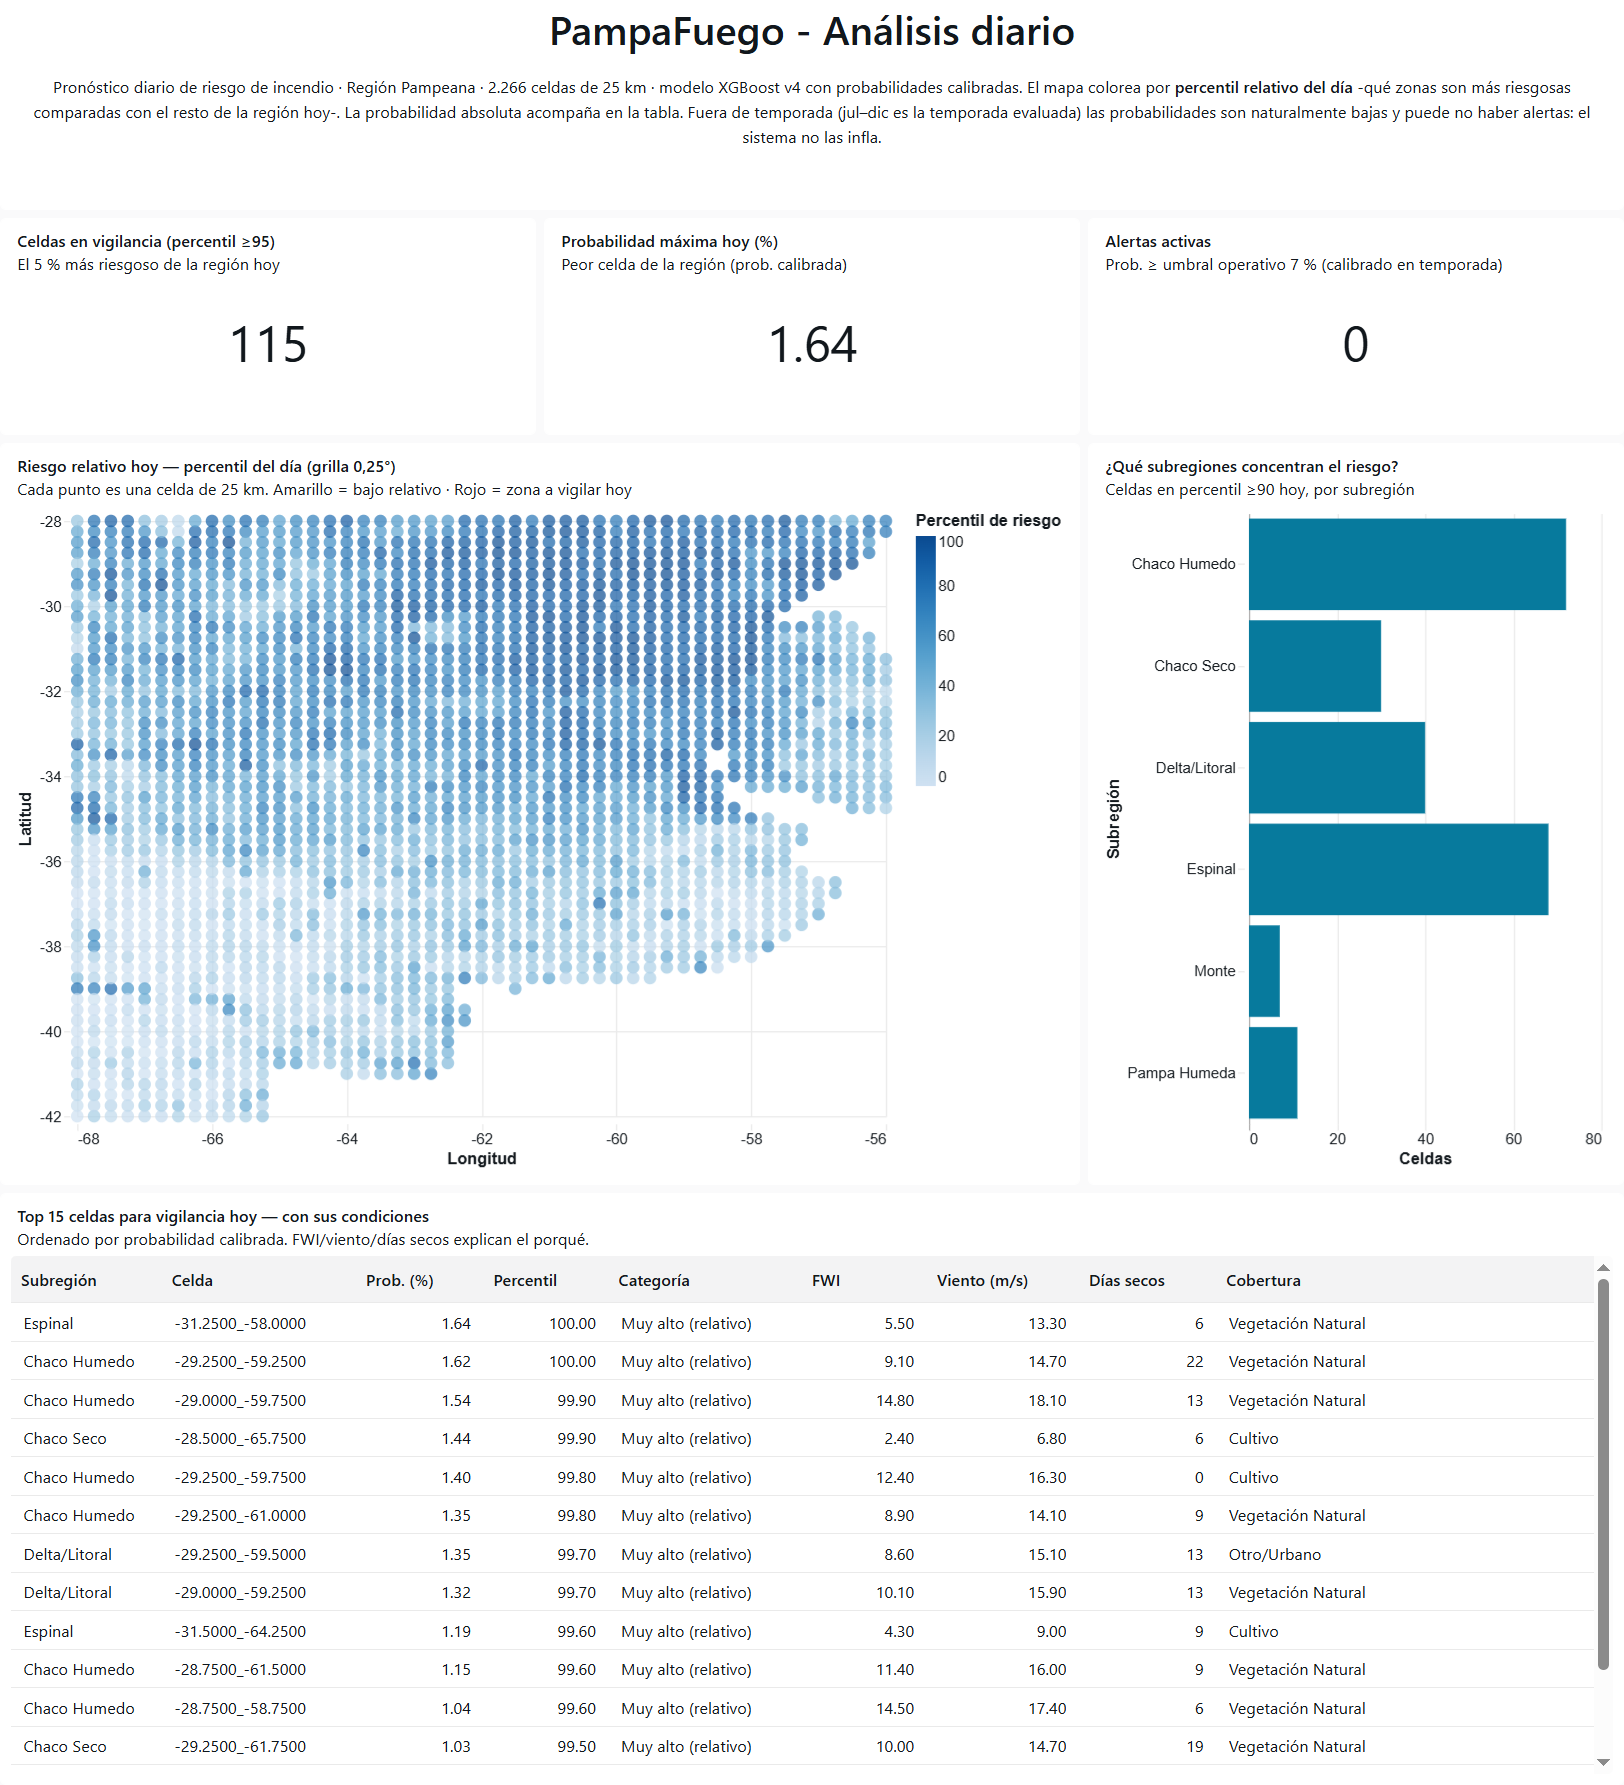
\includegraphics[width=0.82\textwidth,height=0.4\textheight,keepaspectratio]{figures/dash_hoy.png}
\caption{Página principal del tablero operativo. Los indicadores sintetizan
la situación del día, el mapa colorea las 2.266 celdas por percentil de
riesgo relativo y la tabla detalla las quince celdas prioritarias con las
condiciones meteorológicas que explican cada caso.}
\label{fig:dashhoy}
\vspace{7mm}
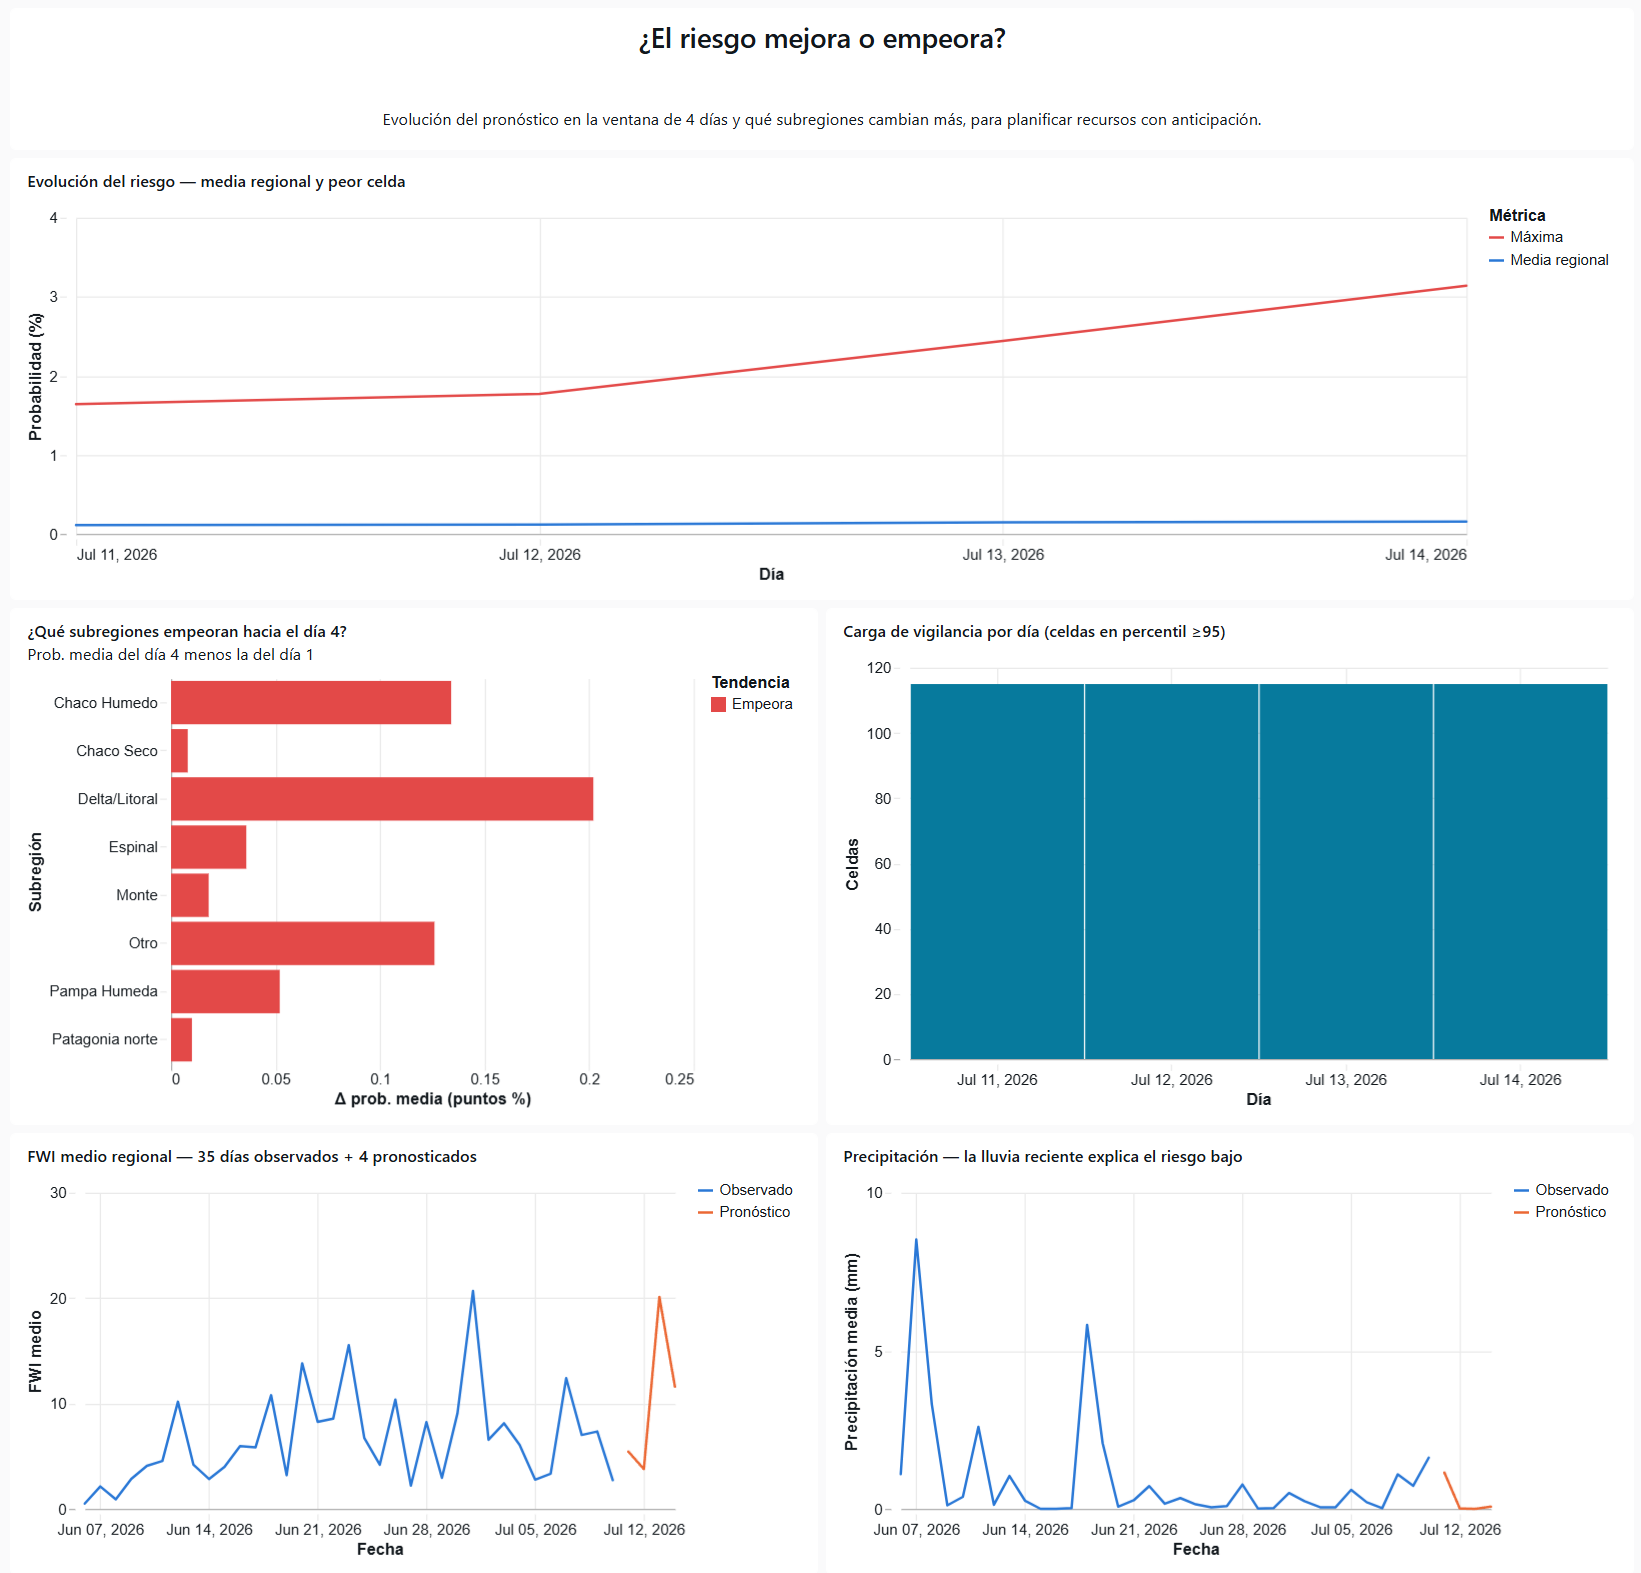
\includegraphics[width=0.82\textwidth,height=0.4\textheight,keepaspectratio]{figures/dash_tendencia.png}
\caption{Página de tendencia del tablero. Evolución de la probabilidad
media y máxima en la ventana de pronóstico, subregiones con mayor
variación hacia el cuarto día y contexto meteorológico de la ventana de 39
días.}
\label{fig:dashtendencia}
\end{figure}}{}

\IfFileExists{figures/dash_modelo.png}{%
\begin{figure}[!t]
\centering
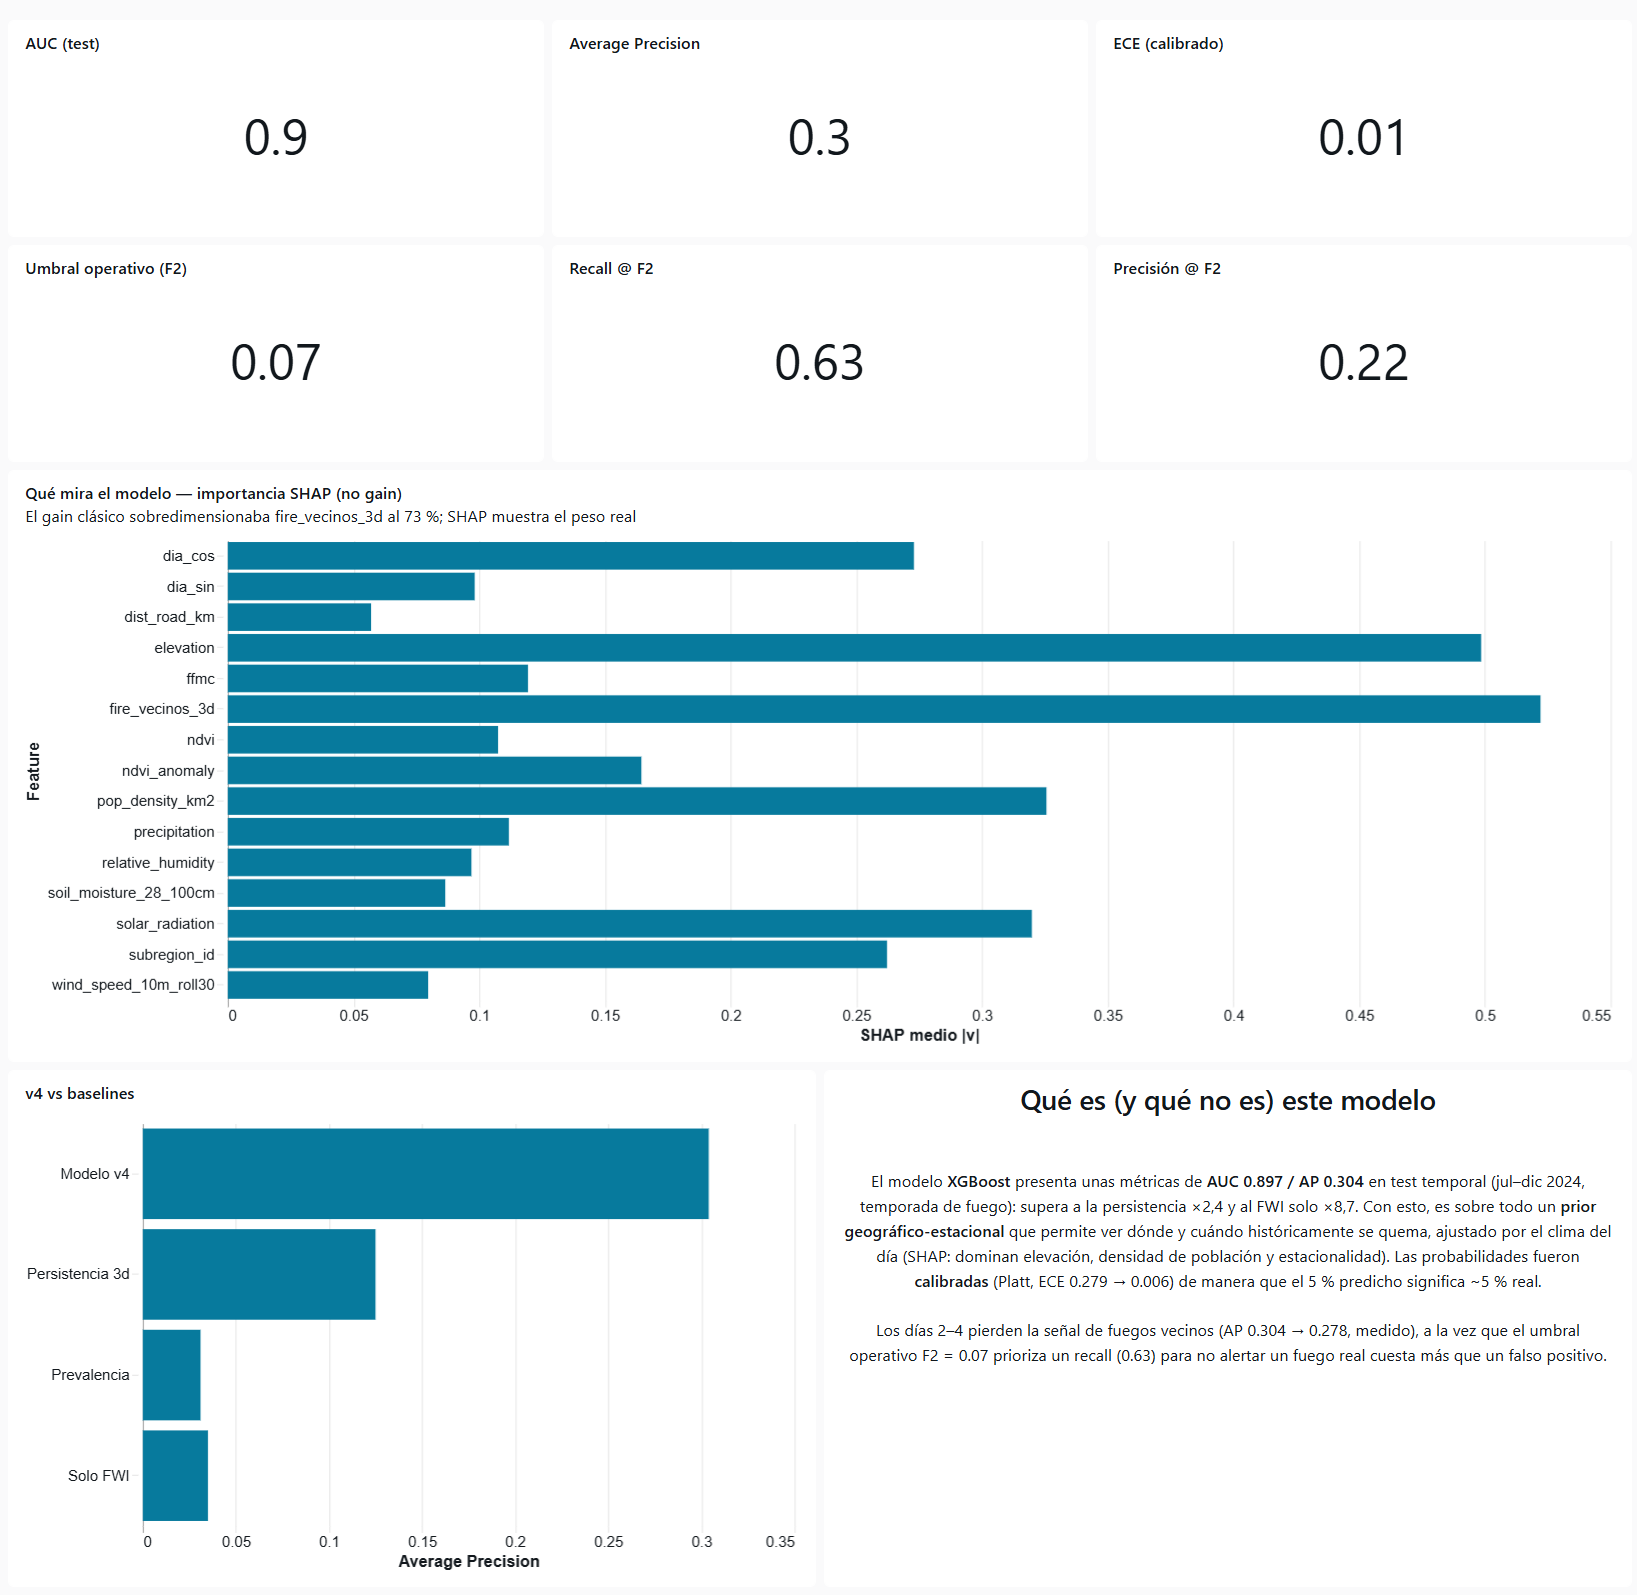
\includegraphics[width=0.82\textwidth,height=0.4\textheight,keepaspectratio]{figures/dash_modelo.png}
\caption{Página del modelo en el tablero. Las métricas de prueba, la
importancia SHAP y la comparación contra líneas de base se exponen al
usuario final como parte de la interfaz.}
\label{fig:dashmodelo}
\end{figure}}{}

\FloatBarrier

% ----------------------------------------------------------------------------
\section{Discusión}
\label{sec:discusion}

\paragraph{Elección del clasificador y del optimizador.}
Los árboles potenciados por gradiente continúan siendo el método de
referencia práctica para datos tabulares estructurados con interacciones no
lineales y volúmenes moderados, y la adopción de SSA mantiene la
comparabilidad con el marco de Wang \emph{et al.}~\cite{wang2026}, cuyo
aporte metodológico central reside precisamente en esa combinación. No se
exploraron arquitecturas de aprendizaje profundo, dado que con
aproximadamente 29.000 ejemplos positivos y variables tabulares la
evidencia disponible no anticipaba beneficios que justificaran el costo
experimental.

\paragraph{Conservación del sistema FWI.}
La ablación demuestra que los índices FWI no aportan capacidad predictiva
en presencia de la meteorología cruda. Se conservan de todos modos en el
sistema por tres razones. Constituyen el lenguaje operativo del dominio,
habilitan la comparación con la literatura y su costo marginal de cómputo
es nulo. La redundancia se documenta explícitamente en lugar de omitirse.

\paragraph{Doble representación en la capa de consumo.}
La coexistencia de la tabla ancha para el modelo y del esquema en estrella
para el tablero responde a que ambos artefactos poseen consumidores y
ciclos de vida distintos. La primera queda ligada al modelo mediante suma
de verificación y garantiza reproducibilidad; el segundo evoluciona con las
necesidades analíticas sin afectar al entrenamiento.

\paragraph{Limitaciones.}
El trabajo presenta limitaciones que conviene explicitar. El denominado
z-score de precipitación de 90 días no constituye el índice SPI estándar de
la Organización Meteorológica Mundial, que requiere una climatología de
treinta años, y debe interpretarse como anomalía relativa dentro del
período disponible. La serie histórica de tres años submuestrea la
variabilidad interanual asociada a ciclos ENSO y sequías plurianuales, y no
se realizó validación cruzada de ventanas deslizantes multianuales. La
variable objetivo corresponde a detección satelital y no a ocurrencia
verdadera, con los falsos negativos de etiqueta que la nubosidad y la
geometría de pasada introducen. La resolución de $0{,}25^{\circ}$ resulta
adecuada para priorización regional pero insuficiente para despliegue
táctico. El cálculo secuencial del FWI se ejecuta celda por celda en un
único proceso, solución suficiente para el dominio actual que requeriría
vectorización distribuida para dominios mayores. Finalmente, el horizonte
operativo se limita a los cuatro días del proveedor de pronóstico, con la
degradación cuantificada en la Sección~\ref{sec:horizonte}.

% ----------------------------------------------------------------------------
\section{Conclusiones}
\label{sec:conclusiones}

Este trabajo construyó y desplegó un sistema completo de predicción diaria
de riesgo de incendio para la Región Pampeana, desde la ingesta de datos
multi-fuente hasta un tablero de decisión operativa. El clasificador
XGBoost optimizado por SSA alcanza un AUC de 0,897 y una precisión media de
0,304 sobre un conjunto de prueba temporal estricto, superando con holgura
a la persistencia espacial y al índice FWI utilizado aisladamente. La
recalibración mediante regresión de Platt reduce el error de calibración en
dos órdenes de magnitud y convierte la salida del modelo en probabilidades
interpretables, condición necesaria para cualquier sistema de alerta que
aspire a la confianza de sus usuarios.

Más allá de las métricas, el trabajo aporta un registro metodológico que se
considera su contribución principal. La documentación de cuatro versiones
del modelo con sus fugas de información y el efecto de corregirlas, la
caracterización del modelo como prior geográfico-estacional mediante SHAP y
ablación, la cuantificación de la degradación por horizonte y la detección
en operación de dos defectos latentes del pipeline mediante contratos de
datos bloqueantes conforman, en conjunto, un argumento empírico a favor de
la ingeniería rigurosa en sistemas de aprendizaje automático aplicado. Las
líneas de trabajo futuro incluyen la validación cruzada temporal multianual
a medida que se acumule historia, el reentrenamiento sin el bloque de
interacciones, la incorporación de una climatología extendida para un
índice de sequía estándar y el aumento de resolución espacial en las
subregiones de mayor riesgo.

% ----------------------------------------------------------------------------
\begin{thebibliography}{12}\small

\bibitem{wang2026}
Wang, H.; Yu, C.; Wang, J.
Spatial Prediction of Forest Fire Risk in Guangdong Province Using
Multi-Source Geospatial Data and Sparrow Search Algorithm-Optimized
XGBoost. \emph{AppliedMath} \textbf{2026}, 6(1), 10.

\bibitem{vanwagner1987}
Van Wagner, C.~E.
\emph{Development and Structure of the Canadian Forest Fire Weather Index
System}; Forestry Technical Report 35; Canadian Forestry Service. Ottawa,
Canada, 1987.

\bibitem{lawson2008}
Lawson, B.~D.; Armitage, O.~B.
\emph{Weather Guide for the Canadian Forest Fire Danger Rating System};
Natural Resources Canada, Canadian Forest Service. Edmonton, Canada, 2008.

\bibitem{chen2016}
Chen, T.; Guestrin, C.
XGBoost: A Scalable Tree Boosting System. En \emph{Proceedings of the 22nd
ACM SIGKDD International Conference on Knowledge Discovery and Data
Mining}, San Francisco, USA, 2016; pp.~785--794.

\bibitem{xue2020}
Xue, J.; Shen, B.
A novel swarm intelligence optimization approach: sparrow search algorithm.
\emph{Systems Science \& Control Engineering} \textbf{2020}, 8(1), 22--34.

\bibitem{platt1999}
Platt, J.
Probabilistic outputs for support vector machines and comparisons to
regularized likelihood methods. \emph{Advances in Large Margin Classifiers}
\textbf{1999}, 10(3), 61--74.

\bibitem{zadrozny2002}
Zadrozny, B.; Elkan, C.
Transforming classifier scores into accurate multiclass probability
estimates. En \emph{Proceedings of the 8th ACM SIGKDD International
Conference on Knowledge Discovery and Data Mining}, Edmonton, Canada, 2002;
pp.~694--699.

\bibitem{lundberg2017}
Lundberg, S.~M.; Lee, S.-I.
A unified approach to interpreting model predictions.
\emph{Advances in Neural Information Processing Systems} \textbf{2017},
30, 4765--4774.

\bibitem{kimball}
Kimball, R.; Ross, M.
\emph{The Data Warehouse Toolkit: The Definitive Guide to Dimensional
Modeling}, 3.ª ed.; Wiley. Indianapolis, USA, 2013.

\bibitem{armbrust2021}
Armbrust, M.; Ghodsi, A.; Xin, R.; Zaharia, M.
Lakehouse: A New Generation of Open Platforms that Unify Data Warehousing
and Advanced Analytics. En \emph{Proceedings of the 11th Conference on
Innovative Data Systems Research (CIDR)}, 2021.

\bibitem{schroeder2014}
Schroeder, W.; Oliva, P.; Giglio, L.; Csiszar, I.~A.
The New VIIRS 375 m active fire detection data product. \emph{Remote
Sensing of Environment} \textbf{2014}, 143, 85--96.

\bibitem{firms}
NASA FIRMS. \emph{Fire Information for Resource Management System}.
Disponible en \url{https://firms.modaps.eosdis.nasa.gov} (acceso julio de
2026).

\bibitem{era5land}
Muñoz-Sabater, J.; \emph{et al.}
ERA5-Land: a state-of-the-art global reanalysis dataset for land
applications. \emph{Earth System Science Data} \textbf{2021}, 13,
4349--4383.

\end{thebibliography}

\end{document}
